\section{Resultados e discussões}
\section{Figuras de Chladni}
%quais fatores influenciam na forma das figuras? Quantas figuras são possíveis?

Ao friccionar o arco de violino contra a placa no ângulo e velocidade corretos, foi possível observar que a areia sobre a placa agitou-se e passou a acumular-se em algumas linhas, formando figuras. Este fenômeno ocorreu em ambas as placas. Cada placa formou padrões diferentes entre si. Além disso, ao excitar a placa em pontos diferentes com o arco, figuras diferentes foram formadas. Também, pressionar o dedo contra a placa em algum ponto ocasionou mudanças na figura. Em particular, o ponto pressionado sempre passa a ser parte de uma das linhas de areia formadas. Dependendo da combinação entre pontos pressionados e posição do arco para excitar a placa, figuras com menos resolução poderiam ser observadas, não formando um padrão claro.

Este fenômeno é explicado pela formação de modos de vibração, no qual as ondas excitadas na placa pelo arrastar do arco de violino têm máxima interferência construtiva. Neste cenário, formam-se ondas estacionárias com pontos da placa tendo deslocamento vertical máximo (pontos de antinós) e pontos na placa com nenhum deslocamento vertical (pontos de nó). Ao vibrar, a placa arremessa a areia, portanto a areia se acumula nos pontos de nós da placa naquele modo de vibração. 

Placas não seguem o padrão de tubos ou cordas de ter modos normais como múltiplos de uma frequência fundamental. Devido à isto, os modos normais não podem ser obtidos através de uma única equação de onda estacionária e a determinação destes modos nem sempre têm solução analítica. Em particular, ao variar os pontos da placa nos quais pressionamos o dedo, variamos às condições de contorno de vibração da placa, forçando a existência de um ponto de nó no ponto em que pressionamos o dedo. Similarmente, ao variar a posição em que o arco é friccionado forçamos a formação de um antinó naquele ponto. A variação dessas condições de contorno altera os modos normais da placa sob estas condições. Portanto, levando em consideração estas condições, é possível variar uma enorme diversidade de figuras em uma mesma placa. 

Indo além, seria possível variar também a placa. Evidentemente, que como a excitação da placa pela fricção com o arco depende da força elástica da placa, isto é, da rigidez do material, esta alteração também fomentaria a formação de outras figuras em comparação à placa inicial em condições de contorno iguais. Por fim, a geometria da placa faz com que as forças atuando sobre cada ponto da placa ao deformar um ponto (pela fricção do arco de violino) também seja diferente visto que a força elástica dependerá da deformação da vizinhança do ponto. E, é em decorrência disto, que foi possível observar a formação de figuras distintas na placa retangular e na placa triangular. 

\section{Tubo de Rijke}
%explique os fenômenos envolvidos neste experimento 
%discuta em termos de similaridades entre o som que sai de tubos fechados e abertos.
%O que muda ao deixarmos o tubo na horizontal ou na vertical?

Ao esquentar a grade de metal e erguer o tubo foi possível ouvir nitidamente um duradouro som em alto volume. Enquanto o som era reproduzido, virar o tubo para posição horizontal resultou na extinção do som. A origem do som emitido tem relação com o sentido de convecção do ar.

Ao aquecer a grade de metal, o ar envolta da grade se expande, ao mesmo tempo, o ar quente se move para cima devido à esta expansão. Ao expandir-se, o ar próximo à grade de metal empurra o ar mais acima, comprimindo-o. Enquanto a vela está aquecendo o tubo, o fluxo de ar que entra é quente, fazendo com que todo ar dentro do tubo se expanda. Porém, ao retirar o tubo de cima da vela, a expansão de ar quente causa uma diminuição na pressão dentro do tubo, por sua vez, esta diferença de pressão entre o interior e exterior do tubo faz com que novas moléculas de ar frio entrem por baixo do tubo. Então, estas novas moléculas entram em contato com a grande quente e se expandem, aquecidas, as moléculas sobem, empurrando e comprimindo o ar um pouco mais frio logo a cima, a menor pressão dentro do tubo faz com que mais moléculas frias entrem e o ciclo se repete periodicamente. Este ciclo de compressão e expansão de ar é o que origina o som. Assim, torna-se evidente que ao virar o tubo na horizontal, a convecção perde a orientação dentro do tubo e o ar quente tende a ir para os dois lados do tubo. Consequentemente, o fluxo de ar perde a propriedade periódica descrita anteriormente e o som é encerrado. Similarmente, ao virar o tubo de ponta cabeça, o fluxo de ar se torna desorganizado, pois a fonte de ar frio está muito distante da grade quente, portanto, o reforço do som não ocorre.

Como o tubo tem as extremidades abertas, sabemos que na extremidade superior, a onda de pressão possui um nó, pois naquele ponto a pressão deve se manter constante e igual à pressão atmosférica. O mesmo ocorre na outra extremidade do tubo. Dessa forma, conclui-se que o som emitido pelo tubo de Rijke é o som emitido por um tubo com duas extremidades abertas. Portanto, as frequências naturais emitidas pelo tubo de Rijke são \(\lambda_n = 2L/n\) em que \(L\) é o comprimento do tubo, pois no comprimento do tubo cabe exatamente meia onda. 

\subsection{Diapasão e coluna d'água}
O experimento do diapasão com coluna de água é uma demonstração clássica da física ondulatória, utilizada para estudar os princípios da ressonância em tubos fechados. No dito experimento, ao colocar diferentes diapasões com frequências diferentes e conhecidas na boca do tubo, fez com que as ondas sonoras se propagassem pela coluna de ar dentro do tubo sendo refletido pelas paredes até a extremidade superior da água, que reflete a onda. 

Para cada diapasão diferente testou-se que, ao variar o nível da água no tubo por completo, ou seja, varia-lo do menor ponto até o maior ponto, observou-se que, em pelo menos um ponto, houve um grande aumento na intensidade sonora, e esse ponto foi demarcado com a descrição da frequência do diapasão que foi usado. Para o melhor tratamento e análise de dados, será aprofundada a discussão quanto aos dados obtidos com o experimento com o diapasão de \qty{512}{Hz}, que poderá ser abrangida para os testes com os outros diapasões.

O experimento com o diapasão de \qty{512}{Hz} apresentou dados singulares, sendo o único que apresentou dois pontos onde houve um grande aumento na intensidade sonora.  Esses dois pontos foram marcados e tiveram suas colunas de ar medidas, como mostrado na \cref{TuboFechado}.
\begin{figure}[H]
	\centering
	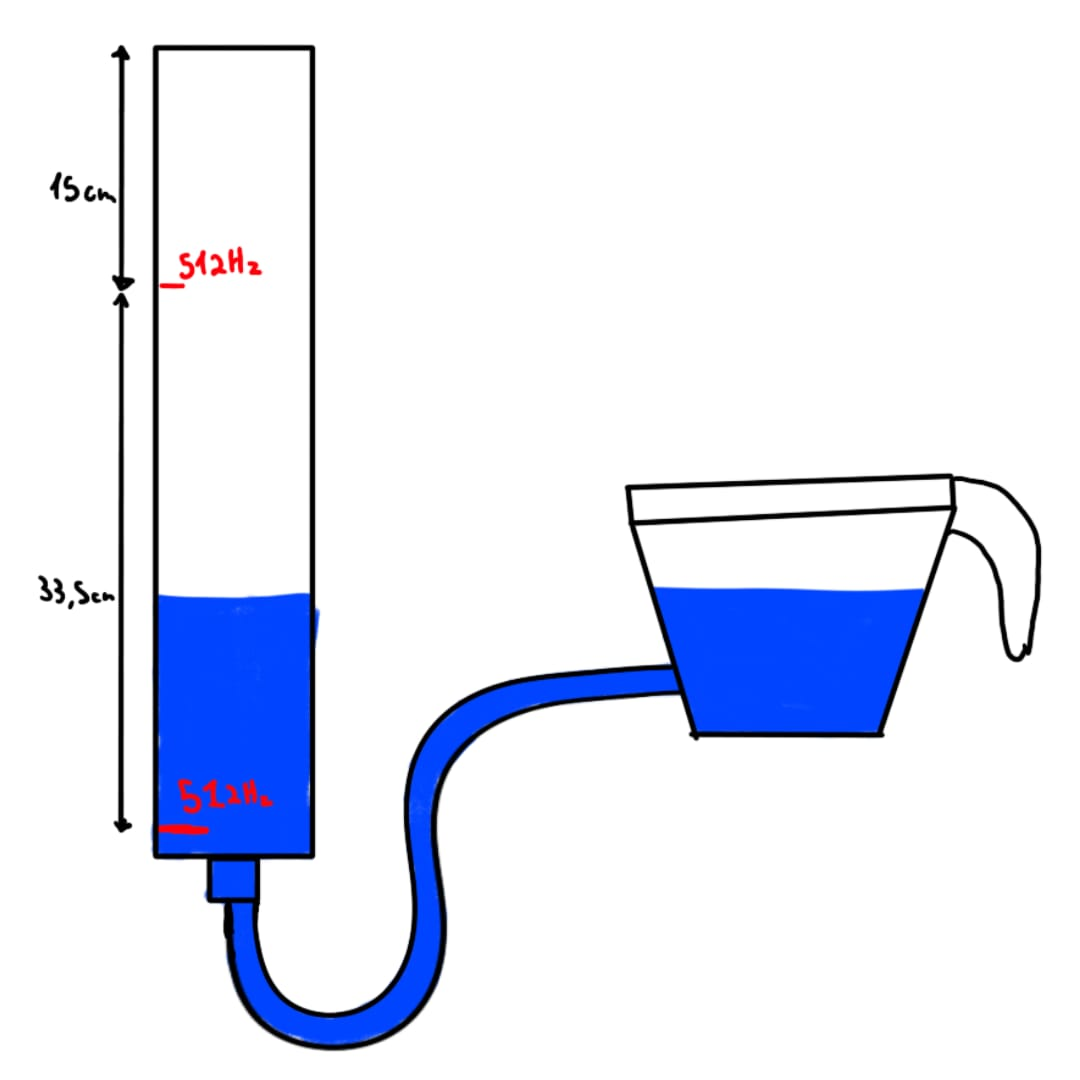
\includegraphics[width=0.35\linewidth]{fig/TuboFechado.png}
	\caption{Tubo de água com uma extremidade fechada e sistema de modificação do nível, marcados e medidos os pontos em que houveram um aumento significativo na intensidade sonora com a vibração de um diapasão de \qty{512}{Hz}. Fonte: Autoria própria.}
	\label{TuboFechado}
\end{figure}

Esse aumento significativo na intensidade do som, ocorre pois quando a onda se propagou pela coluna de ar dentro do tubo, e refletiu-se pela extremidade fechada (superfície da água), criou-se uma \textit{onda refletida} com defasagem de 180º para a onda original, e essa interferência entre as ondas incidentes e refletidas deu origem a uma onda estacionária. Essas ondas estacionárias, são os modos normais de vibração da coluna de ar contida no tubo, que possuem seus pontos de ressonância identificáveis por um aumento significativo na intensidade sonora. E em um tubo com uma extremidade fechada, esses pontos de ressonância ocorrem quando o comprimento da coluna de ar (\(l\)) corresponde a \(\frac{\lambda n}{4}\), para valores impares de n, com n natural, como demonstrado pela imagem \cref{NodoEAntinodo}. 

\begin{figure}[H]
	\centering
	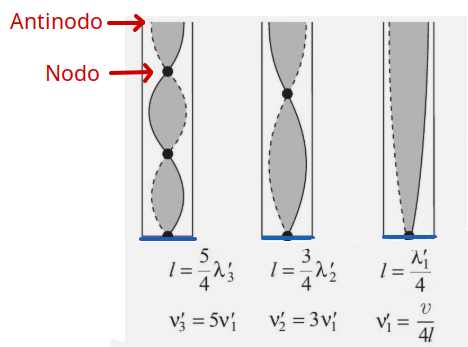
\includegraphics[width=0.35\linewidth]{fig/NodoEAntinodo.png}
	\caption{Demonstração da interferência entre ondas incidentes e refletidas em um tubo fechado, com a formação de nodos e antinodos, posicionados na extremidade fechada e na extremidade aberta, respectivamente, quando as ondas encontram um ponto de ressonância. Abaixo da imagem, formulas de demonstração do tamanho da coluna de ar em que o ponto de ressonância é identificado. Fonte: Modificação de imagem do livro Moyses vol 2.}
	\label{NodoEAntinodo}
\end{figure}

Segundo os dados retirados do experimento, sabe-se que os pontos de ressonância das ondas estacionarias ocorreram com uma coluna de ar de tamanhos \qty{15}{cm} e \qty{48,5}{cm}, possibilitando o calculo do comprimento da onda referente ao primeiro harmônico, que ocorre ao menor \(l\).

\begin{align*}
	l &= \frac{\lambda}{4}\\
	\qty{15}{cm} &= \frac{ \lambda}{4}\\
	\lambda &= \qty{60}{cm} = \qty{0,6}{m}
\end{align*}

Dessa forma, como possui-se o comprimento de onda do som \(\lambda\), e a frequência da onda \(f\), é possível calcular-se a velocidade do som no ar:

\begin{align*}
	v &= \lambda \cdot f\\
	v &= \qty{0,6}{m} \cdot \qty{512}{Hz} \\
	v &= \qty{307,2}{m/s}
\end{align*}

Os resultados experimentais indicaram uma velocidade do som de \qty{307,2}{m/s}, apresentando uma diferença de aproximadamente 10,4\% em relação ao valor teórico de \qty{343}{m/s}. Esta discrepância pode ser atribuída principalmente a: (1) variações nas condições ambientais (temperatura e umidade), já que a velocidade do som varia com a temperatura do ar; (2) imprecisões na determinação do ponto exato de ressonância; e (3) possíveis erros sistemáticos nas medições. Apesar da diferença, o experimento demonstrou ser um método válido para estimativa da velocidade do som em condições controladas.

\subsection{Experimento de Uma Corda}
Este experimento ilustra o princípio de funcionamento dos instrumentos de corda, nos quais o som é produzido pela vibração das cordas. Ao serem colocadas em oscilação, as cordas perturbam o meio ao seu redor, gerando ondas sonoras — variações de pressão que se propagam pelo ar. O perfil dessa oscilação determina as características da onda sonora gerada. Assim, ao alterar propriedades como a frequência ou o comprimento da onda, modifica-se o som produzido.

No experimento de uma corda, observou-se a variação do som emitido pela vibração da corda ao alterar a tensão da mesma. Observando mais especificamente, quando aumentada a tensão da corda, adicionando mais peso a sua extremidade livre, foi possível obter um som mais agudo, ou seja, uma frequência maior.

A explicação dessa alteração de som é sustentada pelas leis das Cordas Vibrantes, descritas por Mersenne. Mais especificamente pela sua segunda lei, que diz, que a frequência fundamental de uma corda é proporcional à raiz quadrada de sua tensão, ou seja, ao aumentar a tensão, aumenta-se sua frequência, e produz um som mais agudo. 

Dessa forma, foi explicado o porquê intrumentos de corda são afinados aumentando a tensão de suas cordas, porém, as leis de mersenne tambpém explicam o porque nesses instrumentos existe a presença de múltiplos tipos de cordas. Segundo as leis de Mersenne, a produção de diferentes sons, a partir de uma corda, pode ser controlada através de três parâmetros principais: (1) a tensão aplicada, (2) o comprimento da corda e (3) suas propriedades físicas. Como o comprimento é limitado pela estrutura do instrumento e a tensão máxima pela resistência do material, a terceira lei de Mersenne oferece uma solução prática: a frequência fundamental é inversamente proporcional à raiz quadrada da densidade linear. Assim, variando a espessura e o material das cordas - e consequentemente sua densidade linear - é possível expandir significativamente a faixa tonal do instrumento. Este princípio é particularmente evidente em guitarras, onde cordas de diferentes calibres (mais finas para agudos, mais grossas para graves) permitem a execução de notas em diversas oitavas.

